\documentclass[10pt]{beamer}
\usepackage{amsfonts, amsmath, amssymb, amscd, amsthm, graphicx,enumerate}
\usepackage[english,main=russian]{babel}
\usepackage{mathrsfs}
\usepackage{comment}
\usepackage{listings}
\usepackage{caption}
\DeclareGraphicsExtensions{.png}
\usetheme{Darmstadt}
\useoutertheme[subsection=false, infolines=false]{miniframes}
\usecolortheme{default}
\usefonttheme[onlymath]{serif}

\captionsetup{justification=centering}



\newcommand{\p}{{\sf P}}
\newcommand{\e}{{\sf E}}
% THEOREM Environments ---------------------------------------------------
\newtheorem{thm}{Теорема}[section]
\renewcommand{\proofname}{Доказательство}
\newtheorem{cor}[thm]{Следствие}
\newtheorem{lem}[thm]{Лемма}
\newtheorem{prop}[thm]{Предложение}
\newtheorem{prob}[thm]{Problem}
\newtheorem{conj}[thm]{Conjecture}
\theoremstyle{definition}
\newtheorem{defn}[thm]{Определение}
\theoremstyle{remark}
\newtheorem{rem}[thm]{Remark}
\newtheorem{ex}[thm]{Example}

\newcommand{\floor}[1]{\lfloor{#1}\rfloor}
\newcommand{\ceil}[1]{\lceil{#1}\rceil}
\DeclareMathOperator{\E}{E}
\DeclareMathOperator{\Var}{Var}
\DeclareMathOperator{\I}{I}
\DeclareMathOperator{\sgn}{sgn}
\DeclareMathOperator{\Law}{Law}
\DeclareMathOperator{\argmax}{arg\,max}
\renewcommand{\hat}{\widehat}
\renewcommand{\tilde}{\widetilde}
\renewcommand{\epsilon}{\varepsilon}
\renewcommand{\P}{\mathrm{P}}
\newcommand{\F}{\mathcal{F}}
\newcommand{\R}{\mathbb{R}}
\newcommand{\bt}{\tilde{b}}
\renewcommand{\b}{\bar b}
\newcommand{\M}{\mathcal{M}}
\let\Ss\S
\renewcommand{\S}{\mathcal{S}}
\newcommand{\cadlag}{c\`adl\`ag}


\makeatletter
\defbeamertemplate*{footline}{my theme}{
	\leavevmode%
	\hbox{%
	\begin{beamercolorbox}[wd=.3\paperwidth,ht=2.25ex,dp=1ex,center]{author in head/foot}%
		\usebeamerfont{author in head/foot}%
		\insertshortauthor
	\end{beamercolorbox}%
	\begin{beamercolorbox}[wd=.5\paperwidth,ht=2.25ex,dp=1ex,center]{title in head/foot}%
		\usebeamerfont{title in head/foot}\insertshorttitle
	\end{beamercolorbox}%
	\begin{beamercolorbox}[wd=.2\paperwidth,ht=2.25ex,dp=1ex,right]{date in head/foot}%
		\usebeamerfont{date in head/foot}
		\insertframenumber{} / \inserttotalframenumber\hspace*{2ex}
	\end{beamercolorbox}}%
}
\makeatother


\begin{document}

\title[Стратегии относительного оптимального роста]{\bf Стратегии относительного оптимального роста в модели рынка с аффинными выплатами\\}
\author[Токаева А.А.]{Токаева Александра Александровна\, \\ научный руководитель\\  к.ф.-м.н.\, Житлухин Михаил Валентинович}
\date{\small{МГУ им. М.В.Ломоносова\\механико-математический факультет\\ кафедра теории вероятностей, 609 группа\\}\vspace{0.5cm} 
Москва\\ \\ 27 мая 2023 г.}

%1------------------------------------------------------------------------------------------------------------------------------------------------------------------------------------

\begin{frame}
  \transdissolve[duration=0.2]
  \titlepage
\end{frame}

%2------------------------------------------------------------------------------------------------------------------------------------------------------------------------------------
\section*{}
\begin{frame}
 \transdissolve[duration=0.2]
 \frametitle{Содержание}
 \tableofcontents
\end{frame}

%3------------------------------------------------------------------------------------------------------------------------------------------------------------------------------------
\section{Введение}
\subsection{Введение}
\begin{frame}\frametitle{Введение} 
    \begin{itemize}

    \item Цель работы — построить стратегию, ``выживающую''  на рынке вне зависимости от стратегий других инвесторов.\\
    \item Стохастическая модель рынка с дискретным временем, эндогенными ценами и аффинными дивидендами.\\
    \item Обобщается модель из статьи Amir R., Evstigneev I., and Schenk-Hoppé K. R.  {\em Asset market games of survival: a synthesis of evolutionary and dynamic games (2013). }
    \item Необходимость рассмотрения такой модели указана в статье Evstigneev I., Hens T., and Schenk-Hoppé K. R. {\em Evolutionary behaviorial finance (2016).} 
    \item Результаты работы изложены в статье Evstigneev I., Tokaeva A., Vanaei M., and Zhitlukhin M. {\em Survival strategies in an evolutionary finance model with endogenous asset payoffs (2023).}
        
	
    
    
    \end{itemize}
\end{frame}

%4------------------------------------------------------------------------------------------------------------------------------------------------------------------------------------
\section{Описание модели рынка}
\subsection{Общая модель}
\begin{frame}\frametitle{Общая модель} 
     \begin{itemize}
	\item $N \geq 2$ агентов.\\
    \item $K \geq 2$ активов, активы ``короткоживущие''.\\
    \item Каждый агент $n$ в каждый момент времени $t$ выбирает вектор долей $\lambda_t^n = (\lambda_{t}^{n,1},\ldots,\lambda_{t}^{n,K})$, в которых он вкладывает свой капитал $W_t^n$ в каждый из $K$ активов в момент времени $t$.\\
    \item Цены устанавливаются эндогенно из условия равенства спроса и предложения на каждый из активов.
    \item Активы платят случайные дивиденды $A_t^k$.
    \end{itemize}
\end{frame}

%5------------------------------------------------------------------------------------------------------------------------------------------------------------------------------------
\subsection{Стратегии}
\begin{frame}\frametitle{Стратегии}
    \begin{itemize}
    \item Стратегия $n$-го агента — это последовательность $\Lambda^n =
    (\Lambda_t^n)_{t=0}^\infty$ измеримых векторнозначных функций 
    \[
    \Lambda_t^n =\Lambda_t^n(\bar s_{t},\bar W_0 , \bar \lambda_{t-1})
    \]
    со значениями в стандартном $K$-симплексе 
    \[
    \Delta^K
    =\{ (a^1, \dots, a^K) \in \R^K_+ : a^1+\ldots+a^K = 1\}.
    \]

    \item $\bar s_{t} := (s_1,...,s_{t})$ — история состояний случайного фактора.  
    \item $\bar W_0 := (W_0^1,...,W_0^N)$ — вектор начальных капиталов.
    \item $\bar \lambda_{t-1} := ( \lambda_0,..., \lambda_{t-1})$, где $ \lambda_s = (\lambda^1_s, \dots, \lambda^N_s )$ — история игры.
    \end{itemize}

\end{frame}

%6------------------------------------------------------------------------------------------------------------------------------------------------------------------------------------
\subsection{Активы с аффинными дивидендами}
\begin{frame}\frametitle{Активы с аффинными дивидендами}
    \begin{itemize}
    \item $W_t = \sum_{n=1}^N W_t^n$ — полный капитал рынка в момент времени $t$.
    \item $\mu_{t}^k = \frac{1}{W_t}\sum_{n=1}^{N}\lambda_{t}^{n,k} W_t^n$ — доля $W_t$, вложенная в $k$-й актив.
    \item $A_{t}^k = A_{t}^k(  \bar s_{t} )$, $k=1,\dots,K$ — дивиденды от единицы актива $k$ в момент времени $t\ge 1$.
   
    \item Дивиденды аффинные:
    $$
    \label{6-A-t-k-affine}
    A_{t+1}^k = \alpha_{t+1}^k + \beta_{t+1}^k \mu_{t}^k,
    $$
    где $\alpha_{t+1}^k$ и $\beta_{t+1}^k$ — произвольные случайные величины вида
    \begin{gather}
    \label{7-alpha-t-k}
    \alpha_{t+1}^k( \bar s_{t+1}) = a_{t+1}^k( \bar s_{t+1}, \bar W_0, \bar \lambda_{t-1}( \bar s_{t-1} )), \\
    \label{8-beta-t-k}
    \beta_{t+1}^k( \bar s_{t+1} ) = b_{t+1}^k ( \bar s_{t+1},\bar W_0, \bar\lambda_{t-1}( \bar s_{t-1} ))
    \end{gather}
    с некоторыми измеримыми неотрицательными коэффициентами $a_{t+1}^k$, $b_{t+1}^k$.
    \end{itemize}
\end{frame}

%7------------------------------------------------------------------------------------------------------------------------------------------------------------------------------------
% \subsection{Динамика капитала}
% \begin{frame}\frametitle{Динамика капитала}
%     \begin{itemize}
%     \item $\bar P_t = (P_{t}^1,\ldots,P_{t}^K)$ — вектор цен активов в момент времени $t$.\\

%     \item $\bar X_t^n=(X_{t}^{n,1},\dots,X_{t}^{n,K})$, где $X_{t}^{n,k}= \frac{\lambda_{t}^{n,k} W_t^n}{P_{t}^k}$ — количество единиц актива $k$ в портфеле.\\

% 	\item  Из равенства спроса и предложения находим цены.\\
%      \[
%     1 = \sum_{n=1}^{N}X_{t}^{n,k} 
%     = \sum_{n=1}^{N}\frac{\lambda_{t}^{n,k}W_{t}^{n}}{P_{t}^k}
%     \Rightarrow  \boxed {P_{t}^k = \sum_{n=1}^{N}\lambda_{t}^{n,k}W_{t}^{n}}
%     \]
    
%     \item Динамика капитала имеет вид
%     $$
%     W_{t+1}^n = \sum_{k=1}^K 
%     X_{t-1}^{n,k} A_{t+1}^k =
%     \sum_{k=1}^K \frac{\lambda_{t}^{n,k} W_t^n}{P_t^k} A_{t+1}^k=
%     \boxed {\sum_{k=1}^K \frac{\lambda_{t}^{n,k} W_t^n}{\sum_{n=1}^N \lambda_{t}^{n,k} W_t^n} A_{t+1}^k}
%     $$
%     \end{itemize}
 
% \end{frame}

%8------------------------------------------------------------------------------------------------------------------------------------------------------------------------------------
\subsection{Выживающие стратегии}
\begin{frame}\frametitle{Выживающие стратегии}
    \begin{itemize}
	\item Мы будем интересоваться поведением \textit{относительных капиталов} агентов, определяемых формулой $r_t^n := \frac{W_t^n}{W_t}.$

	\begin{block}{Определение 1}
    Стратегия $\Lambda^n$ $n$-го агента называется \emph{\bf ``выживающей''}, если для любого вектора начальных капиталов $\bar W_0$ и любого профиля стратегий $\Lambda=(\Lambda^1,\ldots,\Lambda^N)$ с заданной стратегией $\Lambda^n$ и произвольными стратегиями $\Lambda^j$ агентов $j\neq n$ выполняется неравенство $W_t^n > 0$ п.н.\ для всех $t\ge 0$ и 
    \[\inf_{t\ge 0} r_t^n > 0\ \text{п.н.} \]
	\end{block}
    \end{itemize}
\end{frame}



%9------------------------------------------------------------------------------------------------------------------------------------------------------------------------------------
\section{Основные результаты}
\subsection{Теорема 1: ``выживающая'' стратегия — неподвижная точка отображения}
    \begin{frame}\frametitle{Основная теорема (теорема 1)}
    \begin{block}{Теорема 1}
    \label{theorem1-main}
    Пусть $\sum_{k=1}^K (a_{t}^k(\bar s_{t}, \bar W_0, \bar\lambda_{t-2}) + b_{t}^k (\bar s_{t}, \bar W_0, \bar\lambda_{t-2})) > 0.$\\
    Тогда ``выживающая'' стратегия $\Lambda_t^*$ существует.
    \end{block}
    
    ``Выживающая'' стратегия $\Lambda_t^*$ является неподвижной точкой отображения $L_t$, явный вид которого представлен в тексте работы:
    \begin{equation}
    \label{3-lambda-star-fixed-point}
    L_{t}(\Lambda_{t}^*) = \Lambda^*_{t}\ \text{п.н.}
    \end{equation}
    
    
    
\end{frame}



%10------------------------------------------------------------------------------------------------------------------------------------------------------------------------------------
\subsection{Теорема 2: ``выживающая'' стратегия единственна}
\begin{frame}\frametitle{Основная теорема 2}
	\begin{block}{Теорема 2}
    \label{theorem2-convergence}
    Если в профиле стратегий $\Lambda=(\Lambda^1,\dots,\Lambda^N)$ агент $n$ использует стратегию $\Lambda^*$, то при $t\to\infty$ выполнено
    \[ 
    \|\lambda_t^n - \mu_t\| \to 0. 
    \]
    То есть выживающая стратегия в некотором смысле единственна.

\end{block}

\end{frame}

%11------------------------------------------------------------------------------------------------------------------------------------------------------------------------------------
\subsection{Теорема 3: случай н.о.р. коэффициентов}
\begin{frame}\frametitle{Основная теорема 3}
	\begin{block}{Теорема 3}
    Пусть последовательность состояний случайного фактора $s_t$, $t\ge1$ состоит из н.о.р.\ случайных величин, а коэффициенты $\alpha_{t}^k$, $\beta_{t}^k$  зависят только от $s_t$, то есть\ $\alpha_{t}^k = a^k(s_t)$, $\beta_{t}^k = b^k(s_t)$.
    Тогда:\\
    а) ``Выживающая'' стратегия существует и постоянна.\\
    б) Пусть дополнительно $\P(\alpha_{t}^k > 0) > 0\ \text{для всех $k=1,\dots,K$}.$ Тогда ``выживающая'' стратегия единственна в классе постоянных стратегий. При этом ``выживающая'' стратегия оказывается полностью диверсифицированной.\\
    в)  ``Выживающая'' стратегия ``захватывает'' рынок. Другими словами, $r_t^n\to0$ п.н.\ при $t\to\infty$ для любого агента $n$, который использует постоянную полностью диверсифицированную стратегию $\Lambda^n \neq\Lambda^*$.
    \end{block}

\end{frame}



%12------------------------------------------------------------------------------------------------------------------------------------------------------------------------------------
\subsection{Численный пример}
\begin{frame}\frametitle{Численный пример}
    \begin{itemize}
    \item Выплата каждого из двух активов равна либо $1 + \mu_{t}^k$ с вероятностью $p$, либо нулю с вероятностью $1-p$, $p=2/3$.
    \item ``Выживающая'' стратегия $\Lambda^*=(1/2, 1/2)$.
    \item На рынке есть 9 инвесторов со стратегиями $\Lambda^n = (n/10, 1-n/10)$, где $n=1,2,\dots,9$.
    \end{itemize}	

    \begin{figure}
    \centering
    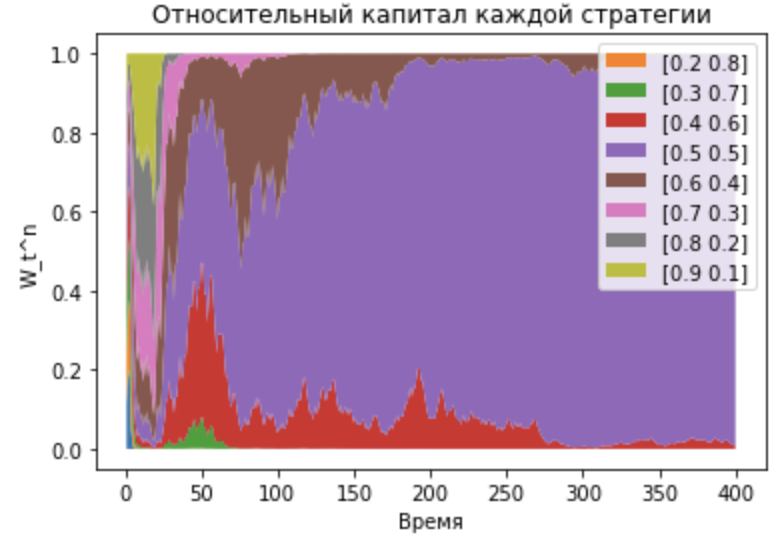
\includegraphics[height=3.5cm]{pictures/pic1-relative-wealth-all.png}\quad
    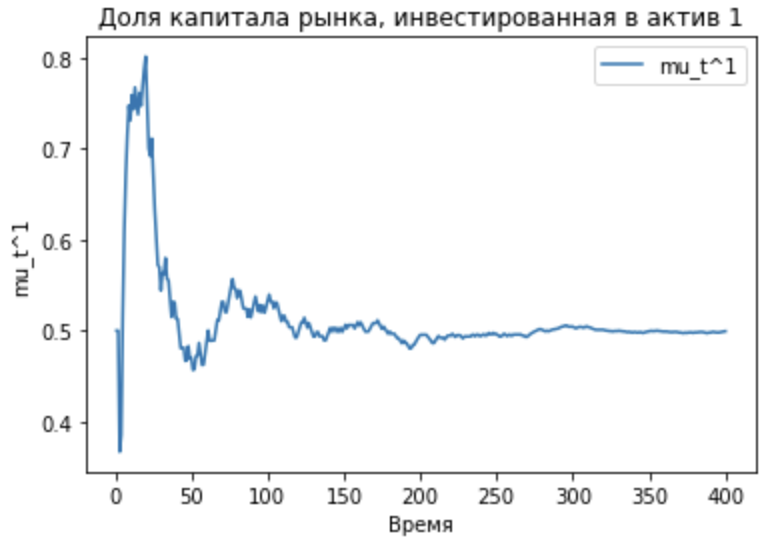
\includegraphics[height=3.5cm]{pictures/pic3-mut1-fraction.png}
     \end{figure}
\end{frame}




%20------------------------------------------------------------------------------------------------------------------------------------------------------------------------------------
\begin{frame}\frametitle{Результаты}
	\begin{enumerate}
		\item{Исследована модель рынка с дискретным временем, эндогенными ценами и аффинными выплатами.}
        \item{Доказаны существование и асимптотическая единственность ``выживающей'' стратегии.}
        \item{Найдены условия, при которых ``выживающая'' стратегия захватывает рынок.}
        \item{Результаты исследования доложены на конференции Ломоносов-2023.}
        \item{Материалы работы вошли в совместную научную статью, которая представлена к публикации в журнале Annals of Operations Research.}
	\end{enumerate}
\end{frame}

%24------------------------------------------------------------------------------------------------------------------------------------------------------------------------------------

\section{Литература}
\begin{frame}\frametitle{Литература}
\begin{thebibliography}{6}



\bibitem{Amir2013} Amir R., Evstigneev I. V., and Schenk-Hoppé, K. R. (2013).
\newblock Asset market games of survival: a synthesis of evolutionary and dynamic games.
{\em Annals of Finance}, 9(2):121–144.


\bibitem{BlumeEasley1992} Blume L. and Easley D. (1992).
\newblock Evolution and market behaviour.
{\em Journal of Economic Theory}, 58(1):9–40.


\bibitem{EvstigneevTokaeva2023} Evstigneev I., Tokaeva A., Vanaei M., and Zhitlukhin M.(2023).
\newblock Survival strategies in an evolutionary finance model with endogenous asset payoffs.
{\em Annals of Operations Research}.


\bibitem{EvstigneevEvolFinance2016} Evstigneev, I., Hens, T., and Schenk-Hoppé, K. R. (2016).
\newblock Evolutionary behaviorial finance. In Haven, E. et al., editors, 
{\em The handbook of Post Crisis Financial Modelling}, 214-234. Palgrave Macmillan UK.


\end{thebibliography}
\end{frame}

%25------------------------------------------------------------------------------------------------------------------------------------------------------------------------------------
\begin{frame}
\center{\Large{Благодарю за внимание!}}
\end{frame}


%-----------------------------------------------------------------------------------------------------------------------------------------------------------------------------------------------------------------------------------------
%Доп1


\begin{frame}\frametitle{Динамика капитала}
    \begin{itemize}
    \item $\bar P_t = (P_{t}^1,\ldots,P_{t}^K)$ — вектор цен активов в момент времени $t$.\\

    \item $\bar X_t^n=(X_{t}^{n,1},\dots,X_{t}^{n,K})$, где $X_{t}^{n,k}= \frac{\lambda_{t}^{n,k} W_t^n}{P_{t}^k}$ — количество единиц актива $k$ в портфеле.\\

	\item  Из равенства спроса и предложения находим цены.\\
     \[
    1 = \sum_{n=1}^{N}X_{t}^{n,k} 
    = \sum_{n=1}^{N}\frac{\lambda_{t}^{n,k}W_{t}^{n}}{P_{t}^k}
    \Rightarrow  \boxed {P_{t}^k = \sum_{n=1}^{N}\lambda_{t}^{n,k}W_{t}^{n}}
    \]
    
    \item Динамика капитала имеет вид
    $$
    W_{t+1}^n = \sum_{k=1}^K 
    X_{t-1}^{n,k} A_{t+1}^k =
    \sum_{k=1}^K \frac{\lambda_{t}^{n,k} W_t^n}{P_t^k} A_{t+1}^k=
    \boxed {\sum_{k=1}^K \frac{\lambda_{t}^{n,k} W_t^n}{\sum_{n=1}^N \lambda_{t}^{n,k} W_t^n} A_{t+1}^k}
    $$
    \end{itemize}
 
\end{frame}

%-----------------------------------------------------------------------------------------------------------------------------------------------------------------------------------------------------------------------------------------
%Доп2


\begin{frame}\frametitle{Выживающая и лог-оптимальная стратегия}
    \begin{itemize}
    \item Чтобы найти выживающую стратегию, мы будем искать \emph{лог-оптимальную стратегию}.
    \end{itemize}
    
    \begin{block}{Определение 2}
    Стратегия $\Lambda^n$ называется \emph{\bf лог-оптимальной }, если  для любого вектора начальных капиталов $\bar W_0$ и профиля стратегий $\Lambda=(\Lambda^1,\ldots,\Lambda^N)$, где $\Lambda^n$ - данная стратегия, выполнено $W_t^n > 0$ п.н.\ для всех $t\ge 0$ и $\ln r_t^n\ \text{является субмартингалом}.$
    \end{block}

    \begin{block}{Утверждение}
    Любая лог-оптимальная стратегия является “выживающей”.
    \end{block}
\end{frame}




    \begin{frame}\frametitle{Утверждение 2}
    \begin{itemize}
    \item $
        g_{t}^k(\lambda^*, \bar s_t, \bar W_0,\bar\lambda_{t-2}) 
        = a_{t}^k(\bar s_t,\bar W_0,\bar\lambda_{t-2}) + \lambda^* b_{t}^k(\bar s_t,\bar W_0,\bar\lambda_{t-2}).
        $

    \item Обозначим $\bar \chi_t=(\bar W_0,\bar\lambda_{t-1}).$
    \item Введем отображение
        \[
        L_{t}^k(\lambda^*, \bar s_t,\bar\chi_t) 
        = \E_t\left(
          \frac{g_{t+1}^k(\lambda^*,\bar s_{t+1},\bar\chi_t)}
               {\sum_{k=1}^K g_{t+1}^k(\lambda^*,\bar s_{t+1},\bar\chi_t)} 
          \right).
        \]
    \end{itemize}

\end{frame}

%-----------------------------------------------------------------------------------------------------------------------------------------------------------------------------------------------------------------------------------------
%Доп3

\begin{frame}\frametitle{Утверждение 2 (продолжение)}
\begin{proposition}
    \label{lemma2-lambda-star}
    Для любого $t\ge0$ существует измеримая функция $\Lambda_t^*(\bar s_t,\bar\chi_t)$ со значениями в  $\Delta^K$ со следующими свойствами:
    \begin{itemize}
    \item для любого $\bar\chi_t$ выполнено:
    \begin{align}
    \label{12-lambda-star-g}
    &\P_t\Biggl(
        \sum_{k=1}^K g_{t+1}^k(\Lambda_t^*(\bar s_t,\bar\chi_t),\bar s_{t+1},\bar\chi_t) = 0
      \Biggr) = 0\ \text{п.н.},\\
    \label{13-lambda-star-inequality}
    &\E_t\left( 
      \frac{b_{t+1}^k(\bar s_{t+1},\bar\chi_t)}
           {\sum_{k=1}^K g_{t+1}^k(\Lambda^*_t(\bar s_{t},\bar\chi_t), \bar s_{t+1},\bar\chi_t)}
      \right) \le 1\ \text{п.н.}, \quad k=1,\dots,K.
    \end{align}
    
    \item $\Lambda_t^*$ — неподвижная точка отображения $L_t$, то есть для любого $\bar\chi_t$ выполнено
    \begin{equation}
    \label{14-lambda-star-fixed-point}
    L_{t}(\Lambda_{t}^*(\bar s_t,\bar\chi_t), \bar s_t, \bar\chi_t) 
    = \Lambda^*_{t}(\bar s_t,\bar\chi_t)\ \text{п.н.}, 
    \end{equation}
    \end{itemize}
    где для $t=0$ полагаем $\Lambda_0^*=\Lambda^*_0(\bar\chi_0)$ зависит только от $\bar\chi_0=\bar W_0$.
    \end{proposition}
\end{frame}


%-----------------------------------------------------------------------------------------------------------------------------------------------------------------------------------------------------------------------------------------
%Доп4



\begin{frame}\frametitle{Основная теорема 2}
	\begin{block}{Теорема 2}
    \label{theorem2-convergence}
    Пусть стратегия $\Lambda^*$ удовлетворяет условиям теоремы 1 и некоторому более сильному условию на функции $g_{t+1}^k$:  существует $\epsilon>0$ такой что для всех $t\ge 0$ и  $\bar \chi_t$ выполнено
    \begin{equation}
    \label{15-lambda-star-inequality-strong}
    \E_t\left( 
      \frac{b_{t+1}^k (\bar s_{t+1},\bar\chi_t)}
           {\sum_{k=1}^K g_{t+1}^k(\Lambda^*_t(\bar s_{t},\bar\chi_t), \bar s_{t+1},\bar\chi_t)}
      \right) \le 1-\epsilon\ \text{п.н.}, \quad k=1,\dots,K.
    \end{equation}
    Тогда, если в профиле стратегий $\Lambda=(\Lambda^1,\dots,\Lambda^N)$ агент $n$ использует стратегию $\Lambda^*$, то выполнено
    \[
    \sum_{t=1}^\infty \|\lambda_t^n - \mu_t\|^2 < \infty\ \text{a.s.},
    \]
    
    В частности, $\|\lambda_t^n - \mu_t\| \to 0$ при $t\to\infty$.

\end{block}

\end{frame}

\end{document}
